% ===================================================================
%  第 5 节 权重二分之一的月光（Moonshine at weight one-half）
%  原文：TASI10.tex 第 1763--2072 行（PDF p.46--p.55）
% ===================================================================
\section{权重二分之一的月光}
\label{sec:Moonshine at weight one-half}

\begin{keytakeaways}
  \item 核心物理图像：$K3$ 椭圆亏格可写成 $\mathrm{EG}(\tau,z;K3)=\frac{\th_1^2(\tau,z)}{\eta^3(\tau)}\big(24\mu(\tau,z)+H(\tau)\big)$，
        其展开系数 $90,462,1540$ 恰为 $2\times(45,231,770)$，而 $45,231,770$ 是 $M_{24}$ 的不可约表示维数；Mathieu 月光正由此发端。
  \item 数学工具：模拟模形式与影子（Appell--Lerch 和 $\mu$ 的模反常与 $H$ 的反常相消）、最优性（optimality）、Rademacher 和、
        Atkin--Lehner 对称性，以及 theta 分解 $\psi^X=\sum_r H^X_r\theta_{m,r}$。
  \item 本影月光的统一构造：23 个 Niemeier 格 $N^X$ 的根系统 $X$ 确定本影群 $G^X=\mathrm{Aut}(N^X)/\mathrm{Weyl}(X)$，
        也确定权重一的最优模拟 Jacobi 形式 $\psi^X$；猜想 \ref{conj:mock_umbral} 断言相应的 $G^X$-模 $K^X$ 存在，其分量为 $K^X_{r,D}$。
  \item Mathieu 月光是本影月光在 $X=24A_1$ 处的实例；$X=12A_2$ 的例子给出 $G^X\cong 2.M_{12}$，
        其分次维数 $16,55,144$ 与 $10,44,110$ 都是不可约表示的维数。
  \item Thompson 月光把 $\Th$ 与权重 $1/2$ 的弱全纯模形式 $f_3$、$\mathcal{F}_3=2f_3+248\theta$ 联系起来；
        猜想 \ref{conj:thompson} 断言存在 $\Th$-超模 $W=\bigoplus_{m\geq-3,\ m\equiv0,1\bmod4}W_m$，其分次超维数给出 $\mathcal{F}_{3,g}$。
  \item 未解问题：对全部 23 个实例统一构造本影模 $K^X$ 仍是月光研究中最大的挑战之一；
        本影月光的判别式性质（判别式 $D$ 与 $K^X_{r,D}$ 中表示的特征标所生成的数域相关）目前尚无物理解释。
\end{keytakeaways}

% [Tutor Note: 2010 年这一波新发展的起点是 Eguchi–Ooguri–Tachikawa 对 $K3$ 椭圆亏格的观察；权重 $1/2$ 之所以最先被开发，是因为 $K3$ 椭圆亏格中的模拟模部分恰好是权 $1/2$、影子为 $24\eta^3$ 的模拟模形式 $H$，而 $K3$ 弦论又提供了现成的物理语境。]

出乎意料的是，2010 年兴起了一波月光研究的热潮，由此发现了更多月光联系的实例。
这些现代实例与第 \ref{cha:weight0} 节讨论的经典月光实例有相似之处，但也有重要差别。
这些实例中的模对象通常是模拟模形式——第 \ref{subsec:MMF} 节引入的模形式的一种重要而自然的推广——而且其权重不为零。
人们最早探索、收获也最丰厚的领域，是权重 $1/2$ 的模拟模形式。
本节将介绍若干把有限群与权重 $1/2$ 的模拟模形式联系起来的月光实例。

\subsection{Mathieu 月光}
\label{subsec:Mathieu}

新型月光的第一个实例——\emph{Mathieu 月光}——始于对 (\ref{second_def_H}) 中引入的权重 $1/2$ 模拟模形式 $H$ 的若干观察；
这与当年对经典 $J$ 函数的观察开启魔群月光的发展如出一辙。
\cite{Eguchi2010} 指出，$H$ 最初的几个 Fourier 系数恰好等于最大散在群 $M_{24}$ 某些不可约表示维数的两倍。
此外，这一观察是在一个有趣的物理背景中作出的；我们下面简要提及，第 \ref{chap:moonshineK3} 节将作更详细的解释。

% [Tutor Note: 原文 p.46 称 $M_{24}$ 为 “the largest sporadic group”，这是笔误：最大的散在群是魔群 $\MM$（阶约 $8\times10^{53}$），$M_{24}$ 只是 Mathieu 群中最大的一个（阶约 $2.4\times10^8$）。译文照原文作“最大散在群”，读者不要据此记结论。]

现在已经清楚：从许多不同的角度看，Mathieu 月光其实应当视为本影月光的一个组成部分；本影月光将在下一小节综述。
不过，Mathieu 月光在本影月光的其他实例中显得格外突出——不仅因为历史，也因为它与 $K3$ 椭圆亏格的直接关联。
因此，我们先单独用一小节讨论 Mathieu 月光，再讨论本影月光。

回忆一下，模拟模形式 $H$ \eq{second_def_H} 可看作来自 (\ref{polar:M24}) 给出的亚纯 Jacobi 形式 $\psi$。
利用 $\psi$ 与 $K3$ 椭圆亏格的关系 (\ref{eq:psi_EGK3})，以及恒等式 $(\theta_{2,1}-\th_{2,-1})(\t,z) =-i \theta_1(\t,2z)$，
我们得到 $K3$ 的椭圆亏格（参见第 \ref{sec:EG} 节）与模拟模形式 $H$ 之间的如下关系：
\be\label{splitEGM24}
{\bf EG}(\t,z;K3) =  \frac{\th_1^2(\t,z)}{\eta^3(\t)} \,\left(24 \,\m(\t,z) + H(\t)\right)~, 
\ee
其中
\be\label{def:mu}
\m(\t,z) = {i \over \theta_{1}(\t,2z)}  {\rm Av}^{(2)}\left[{y+1\over y-1}\right] = \frac{-i y^{1/2}}{\th_{1}(\t,z)}\,\sum_{\ell=-\inf}^\inf \frac{(-1)^{\ell} y^\ell q^{\ell(\ell+1)/2}}{1-y q^\ell}~.
\ee

% [Tutor Note: $\mu(\tau,z)$ 是 Appell–Lerch 和，只是模拟 Jacobi 形式（权 $1/2$），并不满足严格的 Jacobi 形式变换；其模反常的影子的权为 $3/2$（即 $2-1/2$），正是这份反常与 $H$ 的反常相消，才使 ${\bf EG}(K3)$ 成为真正的弱 Jacobi 形式。写 $q$ 展开时注意 $(-1)^\ell y^\ell q^{\ell(\ell+1)/2}$ 的平移项，漏掉它会把影子算错。]

注意，(\ref{splitEGM24}) 右端的两个求和项各自都不作模变换，但它们的模反常相互抵消，左端是一个性质良好的 Jacobi 形式；
第 \ref{sec:modular} 节与第 \ref{sec:EG} 节已讨论过这一点。
特别地，求 $H$ 的影子的一条简便途径，是研究 Appell--Lerch 和 $\mu(\t,z)$ 的模性质 \cite{Eguchi2009a,Zwegers2008}。
第 \ref{sec:M24moonshine}--\ref{sec:umK3} 节将给出 ${\bf EG}(K3)$ 的上述分解 (\ref{splitEGM24}) 的两个有趣的物理解释：
一个用 ${\cal N}=4$ 超共形代数（superconformal algebra）的特征标，另一个用 du Val 奇点的椭圆亏格。

% 原文 p.47 把 superconformal 拼作 “superconfomal”（漏一个 r），译文按正确拼写处理。

% [Tutor Note: $K3$ 椭圆亏格按 $N=4$ 超共形代数特征标展开时，$q^0$ 附近的系数 $90$、$462$、$1540$ 恰为 $2\times(45,231,770)$，而 $45$、$231$、$770$ 正是 $M_{24}$ 的不可约表示维数；因子 2 来自猜想中的“偶表示”条件 $K_n=k_n\oplus k_n^{\,\ast}$。注意 $q^{-1/8}$ 的极项系数 $-2$ 不属于 $K_n$ 的数据，勿把它当作 $\dim K_0$。]

上述观察——模拟模形式 $H$ 的前几个系数与 $M_{24}$ 的某些表示之间存在引人注目的关系——使人猜想：
$H$ 背后存在一个 $\Z$-分次的无限维 $M_{24}$-模 $K= \bigoplus_{n=1}^\inf  K_n$，
即 $H(\t) =q^{-\frac{1}{8}}\big( -2  + \sum_{n=1}^\inf q^n\,({\rm dim}({K_n} )\big)$。
于是自然要问：Jacobi 形式 ${\bf EG}(K3)$ 的分解 (\ref{splitEGM24}) 中的另一项，是否也带有 $M_{24}$ 的作用？
一个简单的猜测来自如下事实：$M_{24}$ 是置换群 $S_{24}$ 的子群，因而有一个 24 维的定义置换表示 ${\bf R}$。
因此，对 (\ref{splitEGM24}) 的“twined”版本，一个自然的提议是
\be\label{K3_EG_Fou}
	 \phi_g(\t,z) 
 		=  \frac{\th_1^2(\t,z)}{\eta^3(\t)} \,\big((\tr_{\bf R} {g } ) \,\m(\t,z) + H_g(\t)\big)~,
	\ee
其中 $H_g$ 记 $M_{24}$-模 $K$ 的分次特征标。
仿照魔群月光的思路，若所有这些 $\phi_g$ 都在某个 $\Gamma_g \subseteq \SL_2(\ZZ)$ 下作为 Jacobi 形式良好地变换，
我们就说存在非平凡的月光联系。第 \ref{sec:orbifolds} 节综述的物理考虑还提示 $ \Gamma_0(|g|) \subseteq \Gamma_g$。

% [Tutor Note: $\Gamma_0(|g|)\subseteq\Gamma_g$ 不是随意假设：orbifold 的 $g$-扭结扇区在 $\tau\to\tau+|g|$ 下不变，因而 twined 配分函数至少对 $\Gamma_0(|g|)$ 协变；$\Gamma_g$ 若比 $\Gamma_0(|g|)$ 更大，则需额外的乘子系统才能一致。]

幸运的是，这类 Jacobi 形式的可能性非常有限，我们只能考虑
\be
\phi = c\, \phi_{0,1} + F \,\phi_{-2,1}~,
\ee
其中 $\phi_{0,1}$ 与 $\phi_{-2,1}$ 由 (\ref{phi01}) 给出，$c\in \CC$；$F$ 是 $\Gamma_g$ 的权重 2 模形式，当 $c=0$ 时可能带有非平凡乘子系统。
对我们关心的 $\SL_2(\Z)$ 子群 $\Gamma_g$，可能的 $F$ 所构成的空间维数往往很小。
例如当 $\Gamma_g = \SL_2(\Z)$ 时，唯一可能的权重 2 形式是 $F=0$。
因此，由前几个 $M_{24}$-表示的猜测所确定的前几个 Fourier 系数，常常足以定出整个函数。

% [Tutor Note: 这里用到 $\SL_2(\ZZ)$ 的权重 2 模形式空间为零，即 $M_2(\SL_2(\ZZ))=0$；对一般的 $\Gamma_0(|g|)$ 该空间可以非零（例如 $\Gamma_0(2)$ 的权重 2 Eisenstein 空间是一维），故 $F$ 一般不为零，正是这些非零的 $F$ 承载了 $M_{24}$ 的表示数据。]

因此，在最初的观察 \cite{Eguchi2010} 之后不久，\cite{cheng2010k3 ,Gaberdiel2010,Gaberdiel2010a,Eguchi2010a}
就对所有共轭类 $[g]\subset M_{24}$ 提出了 McKay--Thompson 级数的候选者，其形式为
\be\label{m24_weakJacform}
{\phi}'_g(\t,z)= \frac{\tr_{\bf R} {g } }{12}\, \phi_{0,1}(\t,z) + \til T_g(\t) \, \phi_{-2,1}(\t,z)~,\;\ee 
其中函数 $\tilde{T}_g(\t)$ 是权重 2 的模形式，在上述文献中有明确给出，并汇总于 \cite{cheng2011largest} 的表 2。
更确切地说，对任意 $g\in M_{24}$，这些 $\phi_g$ 都是权重为零、指标为一的弱 Jacobi 形式，
对一切 $(\l,\m)\in \ZZ^2$ 满足椭圆不变性 $\f_g\lvert_{1} (\l,\m)  = \phi_g$（参见 \eq{elliptic}），并作如下变换：
$$  
{\phi}'_g(\t,z)=\r_{n_g|h_g}(\gamma) \,e\left(-\frac{c z^2}{c\t+d}\right) {\phi}'_g\big({a\t+b\over c\t+d},{z\over c\t+d}\big)~ ,
$$
其中 $\gamma \in\Gamma_0(|g|)$，乘子 $\r_{n_g|h_g}$ 汇总于 \cite{cheng2011largest}。

用弱 Jacobi 形式 (\ref{m24_weakJacform}) 来表述，Mathieu 月光的主要陈述如下。
\begin{conj}\label{conj_mock}
存在一个自然定义的 $\Z$-分次无限维 $M_{24}$-模 $K= \bigoplus_{n=1}^\inf  K_n$，使得对任意 $g\in M_{24}$，分次特征标
\be\label{rep_mock}
H_g(\t) :=q^{-\frac{1}{8}}\big( -2  + \sum_{n=1}^\inf q^n\,(\tr_{K_n} g)\big)
\ee
满足 $\phi_g = \phi_g'$，其中 $\phi_g$ 如 \eq{K3_EG_Fou} 所定义，$\phi_g'$ 是显式给出的弱 Jacobi 形式 \eq{m24_weakJacform}。
此外，表示 $K_n$ 是偶的：它们都可以写成 $K_n=k_n\oplus k_n ^{\,\ast}$ 的形式，
其中 $k_n$ 是某个 $M_{24}$-表示，$k_n ^{\,\ast}$ 是其对偶表示。
\end{conj}

% [Tutor Note: 原文的 label rep_mock 出现了两次（本式 (5.6) 与 5.2 节的本影公式 (5.8)），LaTeX 对重复 label 取“最后定义”，故出版 PDF 中所有 \eq{rep_mock} 都指向 (5.8)。为消除重复定义并恢复本段原意（此处指 Mathieu 情形的 (5.6)），译文把 5.2 节的第二个 label 改为 rep_mock_umbral，并把第 6 节指向本影公式的引用同步改为 rep_mock_umbral；本处引用仍为 (5.6)。]

上述猜想中的关键事实——存在 $M_{24}$-模 $K=\bigoplus_{n=1}^\inf K_n $ 使 \eq{rep_mock} 成立——已在 \cite{gannon2016much} 中得到证明。
然而，与魔群月光中 Frenkel--Lepowsky--Meurman 构造 $V^\natural$ 相仿的对模 $K$ 的构造，至今仍然缺失。
因此我们完全不知道 $K$ 为何应当“自然”。
作为显式数据，$q$ 级数 $H_g(\t)$ 的前几个 Fourier 系数及相应的 $M_{24}$-表示在 \cite{cheng2011largest} 中给出。

注意，上述结论意味着 $K3$ 椭圆亏格的 $q$-、$y$-展开中所有项的背后都有一个 $M_{24}$-超模。
因此人们很自然地想给 McKay--Thompson 级数 $\phi_g$ 赋予物理诠释，把它看作 $K3$ 共形场论的 twined 椭圆亏格（参见 \eq{def:twined_elliptic_genus}）。
这种可能性（或不可能性）将在第 \ref{chap:moonshineK3} 节充分讨论。

% 原文 p.48 把 McKay–Thompson 拼作 “McKay–Thompsen”，译文按正确拼写处理。

% [Tutor Note: 这里 $H_g$ 的影子是 $(\tr_{\bf R}g)\,\eta^3$，权重 $3/2$；$g=e$ 时 $\tr_{\bf R}e=24$，回到 $H$ 的影子 $24\eta^3$。换群元素只按 $(\tr_{\bf R}g)$ 缩放影子的系数，影子的权重始终是 $3/2$（乘子系统则依 $\Gamma_g$ 而变），这份“影子同型”是 Mathieu 月光可行性的关键。]

最后注意，$\phi_g$ 的模形式性质与 $\mu(\t,z)$ 的模拟模性质，立刻给出 $H_g$ 也是模拟模形式。
具体地，它们由
\be\label{h_g_explicit}
H_g(\t) = \frac{\tr_{\bf R} {g } }{24} H(\t) - \frac{\til T_g(\t)}{\eta(\t)^3}~,
\ee
给出，是权重 $1/2$ 的模拟模形式，其影子为 $(\tr_{\bf R} {g } )\eta^3(\t)$；
这推广了 (\ref{completion_H}) 附近讨论的 $H(\t)$ 的模拟模性质。

\subsection{本影月光}
\label{sec:umbral}

Mathieu 月光发现几年之后，人们意识到它其实只是一个更大的月光系统——所谓“本影月光”（umbral moonshine）\cite{UM,cheng2014umbral}——中的一个实例。
本影月光共有 23 个实例，它们具有统一的描述（见图 \ref{UM_construction}）。
本影月光的主要陈述如下。

% [Tutor Note: 原文此处重复使用 label conj_mock（与第 5.1 节相同），会导致编译警告；此处改为 conj:mock_umbral，内容未作改动。]
\begin{conj}\label{conj:mock_umbral}
设 $G^X$ 是 (\ref{eqn:def_um_grp}) 中给出的 23 个有限群之一，$m$ 是 \eq{eqn:Cox_index} 中给出的相应正整数，
$I^X$ 是 \eq{def:setIX} 中描述的 $\{1,2,\dots,m-1\}$ 的特定子集。
则存在一个自然定义的双分次无限维 $G^X$-模 $$K^X=\bigoplus_{r\in I^X} \bigoplus_{\substack{D\leq 0\\ D=r^2\xmod{4m}}}  K_{r,D}^X$$
使得对任意 $g\in G^X$ 及任意 $r\in I^X$，分次特征标（如下文所述，由极项 $ -2 q^{-\frac{1}{4m}}$ 加以“修正”）与向量值模拟模形式 $H^X_g = (H^X_{g,r})_{r\in I^X}$ 的分量 $H^X_{g,r}$ 一致：
\be\label{rep_mock_umbral}
H^X_{g,r} = -2 q^{-\frac{1}{4m}} \d_{r,1} \  + \sum_{\substack{D\leq 0\\ D=r^2\!\!\xmod{4m}}}^\inf q^{-D/4m}\,(\tr_{K_{r,D}^X} g). 
\ee
\end{conj}
下面我们简要说明上述猜想中几个主要角色——有限群 $G^X$ 与模拟模形式 $H^X_g$——的具体设定。参见图 \ref{UM_construction}。

% [Tutor Note: Niemeier 格在 24 维偶幺模正定格中由其根系唯一确定：24 个 Niemeier 格中除无根的 Leech 格外，其余 23 个都有非平凡根系，因此“23 个实例”与“23 个 Niemeier 格”是同一份分类。Leech 格属于 Conway 月光一侧，不在本影月光之列。]

这一统一构造的出发点是第 \ref{sec:sporadic_lattices} 节引入的 23 个 Niemeier 格 $N^X$。
回忆一下，它们由各自的根系唯一标记。
以下用 $X$ 记根系，$N^X$ 记相应的 Niemeier 格，$G^X$ 记由自同构 Aut$(N^X)$ 经 \eq{def:niemeier_grp} 得到的有限群：
\be\label{eqn:def_um_grp}
G^X := {\rm Aut}(N^X)/ {\rm Weyl}(X)
\ee
这些就是与本影月光相关的有限群，我们称之为\emph{本影群}（umbral groups）。

% [Tutor Note: $G^X=\mathrm{Aut}(N^X)/\mathrm{Weyl}(X)$：根格的内自同构（即 Weyl 群）被商掉，剩下的是在根系各分量之间置换的“外”对称性。因此 $G^X$ 只依赖根系 $X$（及其粘合数据），这正是本影群能由 Niemeier 格分类直接读出的原因；估算 $|G^X|$ 时不要忘记 Weyl 群是正规子群。]

在模形式这一侧，我们用根系 $X$ 来指定与有限群 $G^X$ 相关的某些模拟模形式。
为说明其做法，先回忆：魔群月光中的 McKay--Thompson 级数 $T_g$ 与 Mathieu 月光中的模拟模形式 $H_g$ 具有非常特殊的性质。
第一，一旦给定它们的（模拟）模数据（由群 $\Gamma_g$、权重与乘子组成），这些函数就被它们在尖点 $i\infty\cup \QQ$ 附近的增长性质完全确定。
第二，它们具有如下意义的“最优增长”：这些函数 1) 在所有与 $i\infty$ 不 $\Gamma_g$-等价的尖点处有界；2) 在 $i\infty$ 附近的增长是与模数据相容的最慢增长。
例如在魔群月光的情形，容易看出：对 $\Gamma_g\supset \langle T \rangle$，满足条件 1) 的模形式在尖点 $i\infty$ 附近必形如 $q^{-n}(1+ O(q))$，其中 $n$ 为某整数。
于是条件 2) 给出 $n=1$，而月光函数 $T_g$ 确实如此。
上述说法还可以这样表述：魔群月光与 Mathieu 月光中的这些函数（相差一个常数）可由 $i\infty$ 附近展开中最小极项上的 Rademacher 和写出 \cite{DunFre_RSMG,cheng2012rademacher}。
Rademacher 和的讨论另见第 \ref{sec:mm} 节。

% [Tutor Note: 作者说“容易看出”之处，实际论证是：$\Gamma_g\supset\langle T\rangle$ 只保证 $q$-展开在 $q\to q$ 下周期；条件 1) 排除其他尖点处的极项，条件 2) 再把 $i\infty$ 处极项的阶数压到最小。模数据固定后，函数由 Rademacher 和唯一重建——所以“最优增长”实质上是一个存在唯一性定理，而不是渐近估计。]

本影月光的这些函数具有类似的唯一性，这里相关的概念是\emph{最优模拟 Jacobi 形式}（optimal mock Jacobi form）。
我们先考虑 $g=e$、$\Gamma_g = \SL_2(\ZZ)$ 的情形。
设 $\psi=\sum_r h_r\theta_{m,r}$ 是权重为一、指标为 $m$ 的模拟 Jacobi 形式。
若当 $\Im(\t)\to \infty$ 时，对每个 $r\in\ZZ/2m$ 都有
\begin{gather}\label{eqn:intro:opt}
h_r(\tau)=O(q^{-\frac1{4m}})
\end{gather} 
则称它是最优模拟 Jacobi 形式。
例如，第 \ref{subsec:MMF} 节定义的函数 $\psi^{3E_8}$ 就是最优模拟 Jacobi 形式：其指标为 30，
且 $H_1^{3E_8}(\t)= -2q^{-{1\over120}}( 1+O(q))$，而 $H_7^{3E_8}$ 在 $\Im(\t)\to \infty$ 时消失（参见 \eq{eqn:3E8}）。
类似地，$\psi^{24A_1}$ 是指标为 2 的最优模拟 Jacobi 形式。

% [Tutor Note: 这里“最优”（optimal）只要求 $h_r=O(q^{-1/4m})$，即极项取模数据允许的最小阶；再配合模数据，$\psi$ 就由 Rademacher 和唯一确定。经 theta 分解 $\psi^X=\sum_r H^X_r\theta_{m,r}$ 后，$H^X_r$ 是权 $1/2$ 的模拟模形式，其影子是权 $3/2$（即 $2-1/2$）的一元 theta 函数；而 $\theta_{m,r}$ 自身贡献权 $1/2$，两者相加才得到 $\psi$ 的权一，计算时极易把权重弄错。]

在权重一时，这类最优模拟 Jacobi 形式的空间非常受限：
模拟模变换性质连同函数在尖点附近的极点结构，足以确定整个 $q$ 级数。
特别地，它们可以写成只以极部为输入的简单 Rademacher 和。
若还要求 Fourier 系数非超越，这样的形式就更稀少。
注意，函数要在月光中起作用就必须如此，因为分次维数必为整数，当然也是非超越的。
\cite{omjt} 证明：若 $\psi$ 是这种形式，则无论其指标为何，它必落在某个 34 维空间中。
此外，在这个 34 维空间内有 39 个特殊元素（它们张成该 34 维空间），由各自的特殊对称性区分。
回忆一下，使 $\Gamma_0(m)$ 正规化的 Atkin--Lehner 对称性由精确除子群 Ex$_m$ 的一个子群 $K$ 指定（参见 \eq{eqn:groupAL}）。

% [Tutor Note: 39 个特殊元素张成的是 34 维空间，二者数目不等并不矛盾——这些元素线性相关，不要因为出现“39”就以为空间维数是 39。真正能用于月光的 23 个情形，还要额外满足后面的正系数条件。]

给定这样一对 $m$ 与 $K$，称指标为 $m$ 的模拟 Jacobi 形式 $\psi$ 是\emph{$K$-对称}的，如果
\be\label{def:ALsymJac}
\psi = \sum_{r ~ \rm{mod} ~2m} h_r\theta_{m,r}= \sum_{r ~ \rm{mod} ~2m} h_{r}\theta_{m,a(n)r}~~{\text{ 对任意 }} n\in K~,
\ee
其中对给定的 $n$，$a(n)$ 定义为 $\ZZ/2m$ 中唯一满足
\[
a(n) = \begin{cases} 1\xmod{2m/n} \\  -1\xmod{2n}\end{cases}. 
\]
的元素。注意这一对称是对合，因为 $a^2=1\xmod{2m}$。
例如，(\ref{eqn:3E8}) 中引入的模拟 Jacobi 形式 $\psi^{3E_8}$ 在 $K=\{1,6,10,15\}<{\rm{Ex}}_{30}$ 的作用下不变，对应 $a(n)=1,11,19,29$。
\cite{omjt} 中令人惊讶的结果是：一个非零的、$K$-对称的、指标为 $m$ 的权重一最优模拟 Jacobi 形式具有非超越系数，当且仅当相应的 $SL_2(\RR)$ 子群 $\Gamma^{m+K}$ 在上半平面定义一个亏格零商。
回忆一下，这些亏格零群在魔群月光中也扮演重要角色。
注意，为使该模拟 Jacobi 形式非零，我们必须有 $m\not\in K$（称为“non-Fricke”性质），
因为在权重一时 $\sum_{r } h_r\theta_{m,r}=-\sum_{r } h_r\theta_{m,-r}$ 且 $a(m)=-1$。
这样的非 Fricke 亏格零群 $\Gamma^{m+K}<\SL_2(\RR)$ 恰好有 39 个；我们把相应的唯一最优模拟 Jacobi 形式（取如下归一化
\be\label{def:normalisation_um}
h_1 = -2 q^{-\frac1{4m}} (1+O(q) )~,\ee
）记为 $\psi^{m+K}$。

% [Tutor Note: $m\notin K$（non-Fricke）是权一情形特有的条件：由 $\sum_r h_r\theta_{m,r}=-\sum_r h_r\theta_{m,-r}$ 与 $a(m)=-1$ 可知，若 $m\in K$ 则 $\psi$ 恒为零。“Fricke”指的是 Atkin–Lehner 对合中把 $i\infty$ 与 $0$ 互换的那一个，此名源于 Fricke 对 $\Gamma_0(N)$ 的研究。]

事实上，这 39 个特殊的最优模拟 Jacobi 形式 $\psi^{m+K}$ 的 Fourier 系数不仅非超越，而且是整数。
此外，其中 23 个还具有如下意义的正系数。
若写成（参见 \eq{def:thetahat}）
\[
\psi = \sum_{1\leq r\leq m-1}h_r \tilde \th_{m,r}~,\] 其中 $h_r$ 的展开为
\be \label{def:positivity}
h_r = \begin{cases} -2q^{-1/4m}+ \sum_{n\geq 0}c_{r,n} q^{n/4m}  ,~& {\rm{if} }~r^2=1\xmod{4m}  \\ 
\sum_{{n\geq 0}}c_{r,n} q^{n/4m}  ,~& \rm{otherwise }\end{cases}~,
\ee
其中
\(
c_{r,n} \in \ZZ_{\geq0}
\)。
这一正性使得它可以作为有限群表示的分次维数\footnote{据信 \cite{omjt}，其余 16 个系数有正有负的整数最优模拟 Jacobi 形式 $\psi^{m+K}$ 也带有本影型月光，只是需要额外的超模结构来解释那些负号。}。
总而言之，对任意指标，$\SL_2(\ZZ)$ 的权重一特殊模拟 Jacobi 形式共有 23 个，由下列条件刻画：
\vspace{-5pt}
\begin{enumerate}
\item 最优性增长条件 (\ref{eqn:intro:opt}), 
\vspace{-8pt}
\item Atkin--Lehner 对称性 \eq{def:ALsymJac},  
\vspace{-8pt}
\item 归一化 (\ref{def:normalisation_um}), 
\vspace{-8pt}
\item 系数的正性与整性 \eq{def:positivity}.
\end{enumerate}

% [Tutor Note: 39 个非 Fricke 亏格零群中只有 23 个对应的最优模拟 Jacobi 形式具有正整系数，也只有这 23 个能给出月光；其余 16 个系数有正有负，需要额外的超模结构（见脚注）。23 恰与 Niemeier 格数目相同，这是 $\psi^{m+K}$ 与 $X$ 一一对应的关键，并非巧合。]

有趣的观察是：这些具有正性的 $\psi^{m+K}$ 与 23 个 Niemeier 根系 $X$ 一一对应！
为解释这一对应，先回忆 $\widehat{A_1}$ 仿射 Lie 代数模不变组合的 ADE 分类 \cite{Cappelli:1987xt}；
由此得到了具有谱流对称性的 ${\cal N}=2$ 超共形极小模型的分类。
该分类对每个单边（simply-laced）根系 $Y$ 给出一个 $2m$ 阶方阵 $\Omega^Y$，其中 $m$ 恰为 $Y$ 的 Coxeter 数。
此外，项 $(\Omega^Y_{r,r}-\Omega^Y_{r,-r})$ 等于 $r$ 作为 $Y$ 的 Coxeter 指数（不变多项式的次数减一）的重数，取值于 $\{0,1,2\}$。
上述构造可推广到具有相同 Coxeter 数的单边根系之并 $X=\cup_i Y_i$（回忆 Niemeier 根系确实如此），只需定义 $\Omega^X= \sum_i \Omega^{Y_i}$。
于是，对应于 Niemeier 根系 $X$ 的模拟 Jacobi 形式 $\psi^X = \psi^{m+K}$（其 theta 分解为 $\psi^X=\sum_r H^X_r\theta_{m,r}$）与 $X$ 有如下关系。

% [Tutor Note: 指标 $m$ 等于根系 $X$ 的 Coxeter 数：$X=24A_1$（即 $A_1^{24}$）的 Coxeter 数为 2，故 Mathieu 情形的 $q$ 幂次是 $1/(4m)=1/8$；$3E_8$ 的 Coxeter 数为 30，对应 $1/120$。Coxeter 数等于最高根的高度加一，不要与对偶 Coxeter 数（对 $A$、$D$、$E$ 型两者相等，但一般不同）混淆。]

\vspace{-6,5pt}
\begin{enumerate}
\item $X$ 的 Coxeter 数与该 $\psi^X$ 的指标相同，
\vspace{-0,5pt}
\be\label{eqn:Cox_index}
m = {\rm Cox}(X)~.
\ee
\vspace{-25pt}
\item  矩阵 $\Omega^X$ 与形式 $\psi^X=\psi^{m+K}$ 具有相同的 Atkin--Lehner 对称性：
$(\Omega^X)_{r,r'}=(\Omega^X)_{r,a(n)r'}$ 对一切 $n\in K$ 成立。利用这些对称性，可以方便地定义集合 $I^X$：
它是 Atkin--Lehner 对称群作用在 $\{1,\dots,m-1\}$（在 $\ZZ/2m$ 中）上的轨道之集，
用来标记向量值模拟模形式 $(H^X_r)$ 的独立分量 $H_r^X$，并由此得到
\be\label{def:setIX}
\psi^X = \sum_{r\in I^X} H^X_r \sum_{n\in K} \tilde \theta_{m,a(n)r} ~. 
\ee
\vspace{-15pt}
\item $\psi^X$ 的影子由 $\Omega^X$ 决定。更确切地说，$\psi^X$ 的完备化由斜全纯 Jacobi 形式 $\sigma = \sum_r \overline{\theta^1_{m,r}} \O^{X}_{r,r'} \theta_{m,r'}$ 指定（参见 \eq{eqn:jac:mck-hhat} 及其前面的文字）。
\end{enumerate}
\vspace{-6,5pt}

第 \ref{subsec:MMF} 节对 $\psi^{24A_1}$ 与 $\psi^{3E_8}$ 的描述给出了上述构造的例子。
模拟 Jacobi 形式 $\psi^X$ 于是给出向量值模拟模形式 $H^{X} = (H^X_r)$，后者将扮演本影群 $G^X$ 的模的分次维数。
换言之，在猜想 \ref{conj:mock_umbral} 中有 $H^X_r=H^X_{e,r}$。
对 $X=24A_1$ 的情形，这就是我们在第 \ref{sec:modular} 节与第 \ref{subsec:Mathieu} 节讨论过的 Mathieu 月光函数 $\psi^{24A_1}$。
另一个简单的例子是 $X=12A_2$，此时 $\psi^{X} =\sum_{r=1,2} H^X_r\tilde \theta_{3,r}$（于是 $m=3$，$I^X=\{1,2\}$），且
\begin{gather}\begin{split}
H^X_1(\t)& =   2 q^{-1/12} (-1 + 16 \,q+ 55 \,q^2+ 144  \,q^3+\dots)\\ 
H^X_2(\t)& =  2 q^{8/12} (10 + 44 \,q+ 110 \,q^2+\dots) . 
\end{split}
\end{gather}
与此同时，相应 Niemeier 格的对称性给出 $G^X \cong 2.M_{12}$。
有限群 $G^X$ 与向量值模拟模形式 $H^X$ 之间的关系，可以从如下事实看出：群 $2.M_{12}$ 具有维数 $16,55, 144$ 以及 $10,44,110$ 的不可约表示。

% [Tutor Note: $G^{12A_2}\cong 2.M_{12}$ 是 $M_{12}$ 的双重覆盖（Schur 乘子为 $\ZZ_2$）。$H^X_1$ 的系数 $16,55,144$ 与 $H^X_2$ 的系数 $10,44,110$ 分别对应两组不可约表示；$q$ 的幂次以 $1/12$ 为单位（$m=3$），恰好把系数排成分次维数的形式，这是支持本影猜想最直接的数值证据之一。]

\begin{figure}[t]
  \begin{center}
    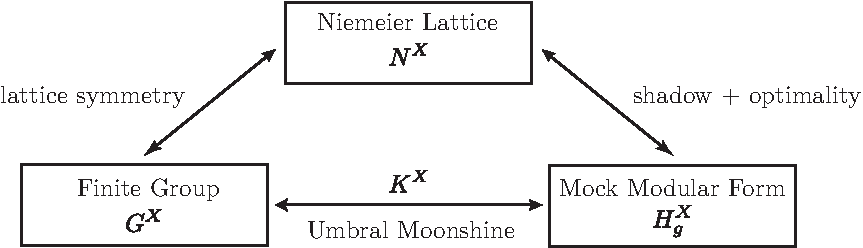
\includegraphics[width=0.92\linewidth]{figures/fig3_umbral_construction.pdf}
    \caption{本影月光的构造。（原文 p.52，图 2）图中：由 Niemeier 格 $N^X$ 的格对称性得到有限群 $G^X$；由影（shadow）与最优性得到模拟模函数 $H^X_g$；下方双箭头即本影月光。}
    \label{UM_construction}
  \end{center}
\end{figure}

指定好 $\SL_2(\ZZ)$ 的模拟 Jacobi 形式之后，为描述月光关系，我们还需要一族模拟 Jacobi 形式
$\psi^X_g= \sum_r H_{g,r}^X\theta_{m,r}$：$\SL_2(\ZZ)$ 的每个子群对应一族，$G^X$ 的每个共轭类 $[g]\subset G^X$ 对应其中一员。
模拟模形式 $H^X_g=(H^X_{g,r})$ 于是扮演本影月光模的分次特征标，如猜想 \ref{conj:mock_umbral} 所述。
这可以在很大程度上仿照 $\SL_2(\ZZ)$ 情形实现，不过会出现额外的微妙之处，需要格外小心。
更多细节参见 \cite{cheng2018weight}。

一旦指定了模拟模形式 $H^X_g$，逐项验证猜想 \ref{conj:mock_umbral} 中 $G^X$-模 $K_{r,D}^X$ 的存在性就是平凡的，即每次只验证一个 $D$。
此外，整个本影模 $K^X=\bigoplus_r \bigoplus_D K_{r,D}^X$ 的存在性，已利用（模拟）模形式的性质得到数学证明 \cite{gannon2016much,DuncanGriffinOno}。
然而，$K^X$ 的构造、甚至对其确切本性的理解，在一般情况下仍然缺失。
迄今只在若干特别简单的本影月光情形中构造出了 $K^X$，对应的 Niemeier 根系为
$3 E_8$ \cite{duncan2017umbral}，$4A_6$ 与 $2A_{12}$ \cite{Duncan:2017bhh}，$4D_6$、$3D_8$、$2D_{12}$ 与 $D_{24}$ \cite{Cheng:2017grj}，以及 $6D_4$ \cite{Anagiannis:2017src}。
\cite{duncan2017umbral} 的构造依赖于模拟模形式 $H^{3E_8}_{g,r}$ 所满足的特殊恒等式，这些恒等式把它与一类格和联系起来；
而 \cite{Duncan:2017bhh,Cheng:2017grj} 则把与 $\Psi^X_{g}$ 相关的亚纯 Jacobi 形式解释为某些顶点算子代数（或手征共形场论）的 twined 配分函数，并用它构造相应的模。
\cite{Anagiannis:2017src} 利用（twined）$K3$ 椭圆亏格、本影月光与 Conway 月光之间的关系，构造了本影月光 $6D_4$ 情形的模；这一关系将在第 \ref{sec:umK3} 节解释。
注意，这是迄今唯一一个构造出来的模，其对应的本影群（嵌入 $\Co_0$ 时）不固定 $\Co_0$ 的 24 维表示中的某个 4-平面。
其意义将在第 \ref{sec:symK3} 节讨论。

% [Tutor Note: 所谓“逐项验证是平凡的”指：每个固定 $D$ 上，$H^X_{g,r}$ 的系数是已算好的非负整数，对照 $G^X$ 的特征标表即可判定该分次分量作为 $G^X$-模存在。真正的困难在于把无穷多个 $D$ 的分量统一成一个自然模 $K^X$——整体存在性要靠 (mock) 模形式的性质（Gannon 与 Duncan–Griffin–Ono 的定理），而统一构造至今没有。]

此外，与第 \ref{sec:mm} 节讨论的广义魔群月光类似的广义本影月光，已在 \cite{GUM} 中建立；
这暗示本影月光模 $K^X$ 上应当存在某些共形场论/模张量范畴结构的要素。
尽管有这些结果，公允地说，给出与本影月光的统一描述相称的本影模的统一构造，仍是当前月光研究最大的挑战之一。

在结束本影月光的综述之前，我们指出本影月光的一个特殊性质，称为\emph{判别式性质}（discriminant property）。
它把判别式 $D$（即 $q$ 级数 $H^X_r$ 中各项 $q^{-D/4m}$ 的幂次）与 $K_{r,D}^X$ 中出现的表示的特征标所生成的数域联系起来。
例如在 $X=24A_1$ 的情形，$H_g= H^{24A_1}_{g,1}$ 中 $q^{7/8}$ 项背后的 $M_{24}$-表示为 $K^{24A_1}_{-7} = \rho \oplus \rho^\ast$，
其中 $\rho$ 是 45 维不可约表示，$\rho^\ast$ 是其对偶表示。
同时，$\tr_\rho g$（从而 $\tr_{\rho^\ast} g$）生成域 $\QQ(\sqrt{-7})$。
只要 $\QQ(D)=\QQ(-7)$，类似关系就随 $q$ 幂次的增大延续下去；而且类似性质对全部 23 个本影月光实例一致成立。
目前人们对此惊人而看似深刻的性质尚无物理上的理解。

% [Tutor Note: 判别式性质说：$q^{-D/4m}$ 项的 $G^X$-表示，其特征标取值落在 $\QQ(\sqrt{D})$ 中；$X=24A_1$、$D=-7$ 时就是 $\QQ(\sqrt{-7})$。这与 Ogg 关于“素数 $p$ 整除魔群阶当且仅当 $X_0(p)$ 亏格为零”的著名观察同一风味：表示论数据“知道”二次域。原文强调目前没有物理解释，勿把它当成已知机制。]

\subsection{Thompson 月光}

Thompson 散在群 $\Th$ 是魔群的一个子群，阶为 $|{\rm \it \Th}|\sim9\cdot10^{16}$，含有 $48$ 个共轭类。
Thompson 月光描述 $\Th$ 的表示论与某些权重 $1/2$ 的弱全纯模形式之间的特殊关系。
它最早在 \cite{Harvey:2015mca} 中讨论，是所谓\emph{斜全纯月光}（skew-holomorphic moonshine）\cite{skew_hol_moonshine} 的第一个实例；
后者把斜全纯 Jacobi 形式与有限群表示联系起来。
关于斜全纯 Jacobi 形式的更多数学与物理信息，参见第 \ref{subsec:shjacobiforms} 节与第 \ref{sec:other_physics} 节。

与 Mathieu 月光和本影月光一样，Thompson 月光把与魔群相联系的有限群（参见第 \ref{sec:sporadic_lattices} 节）与权重 $1/2$ 的模对象联系起来。
不过，它有几处不同。
第一，Thompson 月光中的模对象是模形式，而本影月光中的是影子非零的模拟模形式。
第二，Thompson 月光模带有超结构，即表示带有符号。参见猜想 \ref{conj:thompson}。
话虽如此，这一额外的 $\ZZ_2$-分次结构非常简单，完全由 $m \xmod 4$ 控制，其中 $m$ 是对应于月光函数中 $q$ 的幂次的自然 $\ZZ$-分次。
最后我们指出，Thompson 月光也具有与第 \ref{sec:umbral} 节末尾所讨论的本影月光类似的判别式性质。

% [Tutor Note: 超迹 $\str_{W_m}$ 并非普通迹：在超空间 $\ZZ_2$-分次下它取偶部减奇部。该分次由 $m \bmod 4$ 决定——$m\geq0$ 且 $m\equiv0\bmod4$ 或 $m=-3$ 时为偶，其余为奇；允许的 $m$ 只需 $m\equiv0,1\bmod4$，故奇部（带负号）只出现在 $m\equiv1\bmod4$ 的项上，这正是下面 (5.24) 中 $q^5$ 项系数带负号的原因。]

为了描述 Thompson 月光，我们从如下猜想开始 \cite{Harvey:2015mca}：
{\conj \label{conj:thompson} 存在一个 $\ZZ$-分次 $\Th$-超模（参见 \eq{def:supermodule}）
\begin{equation}
W=\bigoplus_{m\geq-3\atop m\equiv0,1\bmod4}^\infty W_m~
\end{equation}
使得 $W_m$ 的分次维数与某个权重 $1/2$ 的弱全纯模形式 $\mathcal{F}_3$ (\ref{eq:F3}) 之间有关系
\begin{equation}
\mathcal{F}_3(\tau)=\sum_{m=-3\atop m\equiv0,1\bmod4}{\str}_{W_m}(1)q^m~.
\end{equation}
此外，相应的 McKay-Thompson 级数
\begin{equation}
\mathcal{F}_{3,g}(\tau)=\sum_{m=-3\atop m\equiv0,1\bmod4}{\str}_{W_m}(g)q^m~,
\end{equation}
由某些权重 $1/2$ 的弱全纯模形式给出，
且 $\mathcal{F}_{3,e}=\mathcal{F}_3$。
最后，若 $m\geq0$ 且 $m\equiv0\bmod4$，或 $m=-3$，则 $W_m$ 在超空间 $\ZZ_2$-分次下为偶；否则为奇。
}\\

\noindent 下面讨论这一猜想的各个要素。函数 $\mathcal{F}_3$ 定义为
\begin{equation}
\label{eq:F3}
\mathcal{F}_3(\tau):=2f_3(\tau)+248\theta(\tau)~,
\end{equation}
其中 $\theta(\tau)$ 是第 \ref{subsec:modular_forms} 节讨论的 Jacobi theta 函数。
下面说明 $f_3$ 的取法。

把 Kohnen-plus 空间 $M_{1/2}^+$ 定义为这样的全纯函数之集：它们像 $\theta$ 一样变换，
并且在 Fourier 展开 $\sum c(n)q^n$ 中额外满足 $c(n)=0~\forall~n\neq0,1\bmod4$。
可以证明，$M_{1/2}^+$ 其实是一维的，由 $\theta$ 本身张成。
然而，若允许尖点处有极点，就得到 Kohnen-plus 空间中权重 $1/2$ 的弱全纯模形式构成的非平凡空间 $M_{1/2}^{!,+}$。
\cite{Zag_TrcSngMdl} 中，Zagier 为 $M_{1/2}^{!,+}$ 构造了一组无穷维基，由如下（唯一的）函数张成：
\begin{equation}
f_d(\tau)=q^{-d}+\sum_{n>0}A(n,d)q^n~,~~d\equiv0,3\bmod4~,
\end{equation}
其中 $f_0=\theta$。这里我们主要关心 $d=3$ 的情形。

% [Tutor Note: Kohnen-plus 空间的“plus”条件 $c(n)=0$（$n\not\equiv0,1\bmod4$）等价于权 $1/2$ 情形的一个 Fricke 本征条件；正是一维性（$M^+_{1/2}=\CC\,\theta$）与允许尖点极点后得到的 $M^{!,+}_{1/2}$ 里出现 $q^{-3}$ 极项，才使 Thompson 月光能把极项 $2q^{-3}$ 作为 Rademacher 和的唯一输入。]

利用唯一性容易证明，$f_3$ 可显式写成
\begin{equation}
\label{eq:by_hand_f3}
f_3(\tau)=-\frac{1}{20}\left(\frac{[\theta(\tau),E_{10}(4\tau)]}{\Delta(4\tau)}+608\theta(\tau)\right)=q^{-3}-248q+26752q^4-\dots~,
\end{equation}
其中 $E_{10}=E_4E_6$ 是权重 10 的 Eisenstein 级数，$\Delta$ 是第 \ref{subsec:modular_forms} 节引入的权重 12 尖形式。
\emph{Rankin-Cohen 括号}定义为 $[f,g]:=kfDg-lgDf$，其中 $D=\frac{1}{2\pi i}\frac{d}{d\tau}$，$k,l$ 分别是模形式 $f,g$ 的权重。

Thompson 月光始于如下观察：$f_3$ 的前几个 Fourier 系数可以用 $\Th$ 的不可约表示维数表示。
例如 $1=1$、$248=248$、$26752=27000-248$。
值得注意的是，$f_3$ 与 $\Th$ 之间的这一联系早已出现在广义魔群月光的语境中 \cite{DixonL.1988Batb,BorcherdsRichard1995AfoO,MR2904095}，参见第 \ref{sec:mm} 节。
具体地说，$\MM$ 的类 $3C$ 的中心化子同构于 $\mathbb{Z}_3\times\Th$ \cite{conway_norton}，因此扭模 $V^\natural_{3\text{C}}$ 带有 $\Th$ 的自然作用。
相应的扭广义特征标由 $f_3$ 的所谓 \emph{Borcherd's lift} 给出：
\begin{equation}
Z(3\text{C},e;\tau)=q^{-\frac{1}{3}}\prod_{n>0}(1-q^n)^{A(n^2,3)}~.
\end{equation}
但请注意，上述与广义魔群月光的联系只限于 $f_3$ 的系数 $A(n^2,3)$，并不能解释为何其余系数也与 $\Th$ 有关系。

% [Tutor Note: $248$ 是 $\Th$ 最小的非平凡不可约表示维数（也等于 $E_8$ 伴随表示的维数），$27000$ 也是 $\Th$ 的不可约表示维数；$26752=27000-248$ 中的负号不是笔误，而是超迹中奇部的符号，与猜想 \ref{conj:thompson} 的 $\ZZ_2$-分次一致。作者特意选这个例子，是因为三项都直接对应 $\Th$ 的表示维数。]

% 原文 p.54 把 Borcherds 的姓氏拼作 “Borcherd's lift”，译文照录原名，未作改动。

为了做得更好，\cite{Harvey:2015mca} 的想法是“修正”该函数，把 theta 函数 $\theta(\t)$ 的额外贡献纳入进来，转而考虑
\begin{equation}
\mathcal{F}_3(\tau):=2f_3(\tau)+248\theta(\tau)=2q^{-3}+248+2\cdot27000q^4-2\cdot85995q^5+\dots~, 
\end{equation}
它属于 Kohnen-plus 空间。
注意交替的符号对应于猜想 \ref{conj:thompson} 中提到的超空间结构。

Thompson 月光的 McKay--Thompson 级数 ${\cal F}_{3,g}$ 具有与上述非常相似的结构。
概略地说，它们最自然地可看作两项之和
\be\label{thompson_mckaythompson}
{\cal F}_{3,g} = {\text{投影 Rademacher 和}} + \th{\text{ 修正}}~,
\ee
其中第一项是唯一的极项 $2q^{-3}$ 对适当群 $\Gamma_g$ 与乘子系统所作的 Rademacher 和，再投影到 Kohnen-plus 空间；
第二项同样涉及 $\theta(d^2\t)$ 的线性组合，其中 $d$ 是与群 $\Gamma_g$ 相容的某些整数。
更多细节参见 \cite{Harvey:2015mca}，尤其是 \cite{GriffinMichael2016Apot}。

值得注意的是，Thompson 月光中的模对象与所谓的奇异模迹（traces of singular moduli）有密切关系，后者是数论中的重要量。
如第 \ref{subsec:MMF} 节最后一个例子所述，奇异模迹的生成函数具有有趣的模性质 \cite{Zag_TrcSngMdl}。
特别地，有
\begin{equation}
A(n,3)=\frac{1}{\sqrt{n}}\sum_{Q\in\mathcal{Q}_{-3n}/\PSL_2(\ZZ)}\chi_{n,-3}(Q)J(\alpha_Q)~,~~n\in\ZZ_+~,
\end{equation}
它与参与 Thompson 月光的模形式 $f_3$ 的 Fourier 系数一致。
上式中 $\chi_{n,-3}$ 表示某个亏格特征标，其精确定义可在 \cite{Zag_TrcSngMdl} 中找到。
若只跟踪二次型的 $\Gamma_0(N)$-等价类，则同样的奇异模迹关系也可在更高水平上建立。

% [Tutor Note: 这里的 $J$ 是奇异模迹定义中归一化的 $j$-函数（$J=j-744=q^{-1}+O(q)$），$\alpha_Q$ 是二次型 $Q$ 对应的虚二次点；求和跑遍判别式 $-3n$ 的二次型在 $\PSL_2(\ZZ)$ 下的类，$\chi_{n,-3}$ 是相应的亏格特征标。Zagier 定理把这组迹的生成函数识别为 $f_3$，于是数论的类数信息与 Thompson 月光的系数是同一批整数。]
